\documentclass{article}
\usepackage{graphicx,fancyhdr,amsmath,amssymb,amsthm,subfig,url,hyperref}
\usepackage[margin=1in]{geometry}
\usepackage{xltxtra}
\usepackage{xgreek}
\usepackage{amsfonts}
\usepackage{amssymb}
\usepackage{amsmath}
\usepackage{amsthm}
\usepackage{mathtools}

\usepackage{caption}
\usepackage{ subfig}
\setmainfont[Mapping=tex-text]{Times New Roman}
%----------------------- Macros and Definitions --------------------------

%% FILL THIS OUT
\newcommand{\studentname}{Νικόλαος Ζαρίφης}
\newcommand{\suid}{03112178}
\newcommand{\exerciseset}{Exercise Set 1}
%% END



\renewcommand{\theenumi}{\bf \Alph{enumi}}

%\theoremstyle{plain}
%\newtheorem{theorem}{Theorem}
%\newtheorem{lemma}[theorem]{Lemma}

\fancypagestyle{plain}{}
\pagestyle{fancy}
\fancyhf{}
\fancyhead[RO,LE]{\bfseries\large NTUAthens}
\fancyhead[LO,RE]{\bfseries\large Θεωρία γράφων}
\fancyfoot[LO,RE]{\bfseries\large \studentname: nick.zarifis@hotmail.com}
\fancyfoot[RO,LE]{\bfseries\thepage}
\renewcommand{\headrulewidth}{1pt}
\renewcommand{\footrulewidth}{1pt}

\graphicspath{{figures/}}
\usepackage{tikz}
%-------------------------------- Title ----------------------------------

\title{Θεωρία γράφων \\ \exerciseset}
\author{\studentname \qquad  ID: \suid}

%--------------------------------- Text ----------------------------------
\DeclarePairedDelimiter\floor{\lfloor}{\rfloor}
\newtheorem{lemma}{Lemma}
\begin{document}
\maketitle
\section*{Άσκηση 1}
	Παίρνουμε το γράφημα $C_{2a}$ αυτό έχει ακτίνα  κι διάμετρο ίση με α. Τώρα κάνουμε την ακόλουθη κατασκευή, πάμε κι βάζουμε ανάλογα πόσο θα αυξήσουμε το β ένα μόνοπάτη $P_k$ πάνω σε μια κορυφή, αυτό έχει ως αποτέλεσμα θα αυξηθεί η διάμετρος κάτα κ. αλλά η ακτίνα δεν αλλάζει όσο το $k \le a$. Και έτσι έχουμε την κατασκευή μας.
	\section*{Άσκηση 2}
	Θα αποδείξουμε ότι δεν ισχύει η άρνησή της. Δηλαδή ότι υπάρχει ζεύγος (r,s) τω για κάθε n και γράφημά με n κορυφέςνα ισχυεί $\Delta(G)<r ,diam(G)<s$. Ας πάρουμε ένα γράφημα με $\Delta(G)=r-1$ . Τότε κάνοντας decomprasion τις αποστάσεις μας έχουμε ότι για αυθαίρετο n στο πρώτο σύνολο με απόσταση 1, θα έχουμε το πολύ r-1 κορυφές . Στο δεύτερο αν υπάρχει το πολύ $(r-1)^2$ κτλπ, Οπότε αν θέσουμε ν=$\frac{(r-1)^s-1}{r-2} +1$ θα έχουμε συνολικά s σύνολα πράγμα άτοπο από υπόθεση. Φυσικά για μικρότερο μέγιστο πλήθος ακμων δεν χρειάζεται να το δείξουμε γιατί απλά μικραίνει η μέγιστη πληρθηκότητα του κάθε συνόλου.
	\section*{Άσκηση 3}
	$\rightarrow$ \\
	Έστω 3ης κορυφές. u,v,w. Παρακάτω βλέπουμε όλες τις πιθανές συνδέσεις τους.
	\begin{figure}[ht!]\centering
		\subfloat {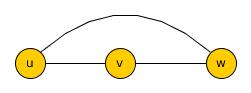
\includegraphics[width=70pt,height=70pt]{ex31}}
			\subfloat {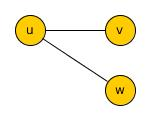
\includegraphics[width=70pt,height=70pt]{ex32}}
				\subfloat {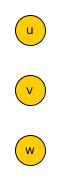
\includegraphics[width=70pt,height=70pt]{ex33}}
	\end{figure}
	Παρατηρούμε  πως αν έχουμε την πρώτη περίπτωση τότε απλά βάζουμε τις 3ης κορυφές σε διαφορετικά σύνολα κι αφού συνδέονται όλα μεταξύ τους είναι ενα πλήρες υποσύνολο, στην δεύτερη περίπτωση απλά οι 2 κορυφές ανοίκουν στο ίδιο σύνολο κι στην τελευταία κι οι 3ης. .Έτσι αφού κάθε μη γειτονικές ακμές έχουν τους ίδιους γείτονες(ολες τις κορυφες που δεν ανοικουν στο ιδιο συνολο)(όπως βλ´επουμε σε οποιοδήποτε υποσύνολο 3ων ακμών), έτσι είναι ένα πλήρες κ-μερες.
	
	$\leftarrow$ Αν εχουμε ενα πληρες κ-μερες τοτε αν απο ενα συνολο κορυφων δεν υπαρχουν οι 2 ακμες τοτε σιγουρα δεν υπαρχει κι η 3η εξ-ορισμου του πληρες κ-μερες
	\section*{Άσκηση 4}
	Φτάνει να δείξουμε ότι κάθε 2 κορυφές ανήκουν σε έναν κοινό κύκλο. Περίπτωση 1:
    Αν δεν είναι γειτονικές τότε λόγο τις ανησώστητας θα έχουμε ότι τουλάχιστον μια απο αφτες έχει $d(v)>n/2$ Όμως όλες οι κορυφές ενδιάμεσα είναι το πολύ n-2 άρα από θεώρημα περιστερώνα θα (ν περιστέρια σε ν-2 φολίες) θα έχουμε ότι οι 2 κορυφές έχουν 2 άλλες κορυφές ενδιάμεσα που τις συνδέουν => Κύκλος.
    Περίπτωσή 2: Αν είναι γειτόνικες τότε αναγώμαστε σε έναν απο τους κύκλους που σχηματίζονται με τις ύπολοιπες κορυφές κι θα περιέχονται αναγκάστηκα κι οι 2 αυτές κορυφές.Αυτό γίνεται διαλέγοντας μια κορυφή που να μην συνδέαιτε τουλάχιστον με την μια.Αν δεν υπάρχει πάλι έχουμε 2 διαφορετικά μονοπάτια ($K_3$). Κι απο το πρώτο ερώτημα θα έχουμε οτί θα υπάρχει κύκλος από αυτή την κορυφή προς την άλλη. Άρα θα έχουμε 2 μονοπάτια, το ένα του κύκλου κι το ένα της σύνδεσεις μεταξύ τους.
    \section*{Άσκηση 5}
    \begin{itemize}
    	\item i 
    	Παίρνουμε το $P_{2k+1}$ και το φτιάχνουμε ακόλουθος:\\
    	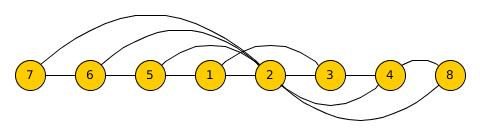
\includegraphics[width=120pt,height=120pt]{ex51} 
    	Τώρα αν αφαιρέσουμε την κορυφή 2, τότε το rad θα αυξηθεί κατά κ , όπως είναι λογικό.
    	\item ii
    	Υποθέτω ότι η εκφώνηση έχει τυπογραφικό λάθος.
    	Αν αφαίρεσω μια κορυφή που δεν ειναι τομής το λιγότερο που μπορεί να μειωθεί το rad είναι κατά 1 αν αφαιρέσω την πιο μακρινή κορυφή κι είναι μοναδική.Αλλίως αφού είναι συνεκτίκο είτε θα είναι σταθερό είτε θα μεγαλώσει. 
    	\item iii
    	Έχουμε από το προηγούμενο ερώτημα ότι $rad(H-u) \ge r-1$ .Αφού είναι το ελάχιστο υπογράφομαι αφαιρώντας μια κορυφή το rad θα μεταβληθεί, αν μεγαλώσει τότε στο γράφημα που μας μένει μπορούμε να αφαιρέσουμε τις πιο μακρινές κορυφές έτσι ώστε το $rad(G1)=r$ όμως αυτό αντιβαίνει ότι το H ήταν το ελάχιστο, πράγμα άτοπο. Άρα μικραίνει κι η ανισότητα γίνεται ισότητα.
    \end{itemize}
      \section*{Άσκηση 6}
      Ξέρουμε ότι $\kappa(G)\le \lambda(G) \le \delta(G)= n$
      Άρα φτάνει να δείξω ότι ισχύει $\kappa(G) =n$. Επαγωγικά, για n=2 ισχύει τετριμμένα (κύκλος.) .Για P(n) ισχύει. Τώρα για το P(n+1) θα εργαστούμε ακολούθως, ξέρουμε ότι σε ένα υπερκύβο οι κορυφές είναι έτσι συνδεδεμένες ώστε να μπορούμε να δημιουργούμε δυαδικές ακολουθίες με τέτοιο τρόπο ωστε κάθε γειτονική κορυφή να έχει διαφορά ένα flip-bit. Άρα ξέρουμε Ότι στα στον $Q_n$ έχουμε ν-ανεξάρτητα μονοπάτια, στον ν+1 έχουμε τα ν απο πριν + ένα μονοπάτι από 2 τυχαία x,y που δημιουργήτε ακολούθως: κάνουμε flip το πιο σημαντικό bit ακολουθούμε μια οποιαδήποτε διαδρομή μέχρι να φτάσουμε στο y με διαφορετικό σημαντικό bit όπου τοε το κάνουμε flip κι φτάσαμε στο προορισμό μας με ένα παραπάνω ανεξάρτητο μονοπάτι, άρα απο Μαθηματική επαγωγή έχουμε ότι ισχύει.
    \section*{Άσκηση 7}
    Ξέρουμε ότι υπάρχουν  τουλάχιστον κ(G) διακεκριμένα μονοπάτια από 2 κορυφές.Παίρνωντας το μεγιστοτίκο μονοπάτι ξέρουμε ότι έχει $diam(G)-1$ κορυφές, επί το πλήθος των μονοπατιών k(G) και προσθέτουμε κι της 2 αυτές κορυφές , καταλήγουμε ότι $n\le k(G)(diam(G)-1) +2$ . Η ανισότητα λόγο του τουλάχιστον.
     \section*{Άσκηση 8}
     Ξέρουμε από θεώρημα menger ότι ανάμεσα σε οποιαδήποτε κορυφές έχουμε 3 διακεκριμένα μονοπάτια. 
     \begin{itemize}
     	\item
     	Τα μονοπάτια έχουν διαφορετικό μήκος κι τελειώσαμε.
     	\item
     	Τα μονοπάτια έχουν ίδιο μήκος. Τότε παίρνουμε απο τα 2 μονοπάτια 2 κορυφές που ισαπέχουν απο το ένα τέρμα.
     	Τώρα από θεώρημα menger πάλι, θα έχουμε πάλι 3 διακεκριμένα μονοπάτια  κι απο περιστερόνα ότι ένα απο αυτά δεν θα περνά απο τα 2 άκρα. Τώρα διακρίνουμε 2 περιπτώσεις. Ή θα συνδεεται άμεσα από το δεύτερο μονοπάτι κι έτσι πέρνοντας το ενδιαμέσο μονοπάτι δημιουργούμε ένα μονοπάτι κι απο τις δύο κορυφές μεγαλύτερου μηκους κι έχουμε κι το τρίτο. Στην δεύτερη περίπτωση , ας ονομάσουμε Χ,Υ τα δύο σημεία που ίσαπεχουν απο το τέλος.ΣΕ αυτή την περίπτωση περνά απο ένα σημείο Κ του τρίτου μονοπατιου. Τώρα έχουμε 2 επιλογές είτε θα πάρουμε το μονοπάτι που σχηματίζεται με αυτές κι κρατάμε το πρώτο μονοπάτι(Κ στο Χ) ή θα πάρουμε το μονοπάτι απο το Κ στο Υ. Γενικά Αν το Κ ισαπέχει απο το τέλος τότε είναι ομοίος με πριν.Αν το Κ δεν ίσαπεχει και δημιούργει το έσωτερικο κι άλλο μονοπάτι ίδιου μήκους τότε το ενώνουμε με το Υ.
     	\end{itemize}
     	 \section*{Άσκηση 9}
     	 Καταρχάς είναι εύκολο να αποδείξουμε ότι κάθε συνεκτική συνηστώστα έχει diam(G)=1 το οποίο μάλιστα σημένει ότι είναι ισομορφικό με ένα $K_n$ .Αυτό τώρα ισχυεί γιατί αν diam($G_i$)>1 τοτε θα μπορούσαμε να πάμε σε μια άλλη συνεκτική συνιστώσα με  diam($G_i$) +1 βήματα γιατί περνάμε κι την γέφυρα όμως αυτό είναι άτοπο γιατί diam(G)=2. Άρα αφαίρωντας την συνεκτικότητα κάθε σύνολο είναι ισομορφισμό με κλίκα(συγκεκριμένα με το βαθμό των κορυφών). Και αν καποιο συνολο περιέχει μια κορυφή προφανές είναι με το $K_1$.
     	 \section*{Άσκηση 10}
     	 	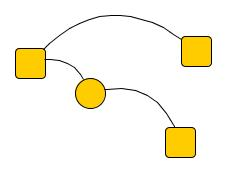
\includegraphics[width=120pt,height=120pt]{ex10}
	     	 	Κάθε τετράγωνο είναι μια συνηστώστα του $K_{c+1}$ . Έτσι ενόνουμε την πρώτη με την δεύτερη με b ακμές σε διαφορετικές κορυφές κι έτσι έχουμε δημιουργήσει κι το επιθυμιτό λ(G).Τέλος ένονουμε τις τελευταίες δυο έτσι ώστε να έχουμε κορυφές ενδιαμέσα πληους α κι να ένονονται με διαφορετικές κορυφές. Επίσεις προσθέτουμε ακμές με τις ενδιάμεσες-συνδετικές κορυφές ώσες χρειάζονται ώστε να μην μικρήνει το λ(G), μιας κι δεν επηρεάζει το κ(G).
	     	 	
 \end{document}
